In exercise-2.1.1 to exercise-2.1.4, rewrite the linear function in slope-intercept form. Then identify the slope and vertical intercept.

\begin{exercise}\label{exercise-2.1.1}
$\displaystyle f(x)=5x-2(x+3)$
\end{exercise}

\begin{solution}
    $f(x)=3x-6$; slope: 3; vertical intercept: $-6$
\end{solution}




\begin{exercise}
$\displaystyle g(x)=4(2x-1)+2$
\end{exercise}

\begin{solution}
    $g(x)=8x-2$; slope: 8; vertical intercept: $-2$
\end{solution}




\begin{exercise}
$\displaystyle h(t)=\frac{18t-5}{2}$
\end{exercise}

\begin{solution}
    $h(t)=9t-2.5$; slope: 9; vertical intercept: $-2.5$
\end{solution}




\begin{exercise}\label{exercise-2.1.4}
$\displaystyle m(x)=2(x-1)+2$
\end{exercise}

\begin{solution}
    $m(x)=2x$; slope: 2; vertical intercept: 0
\end{solution}






 In \exrange{exercise-2.1.5}{exercise-2.1.10}, find the slope of the line passing through each pair of points.

\begin{exercise}\label{exercise-2.1.5}
$(0,10)$ and $(3,16)$
\end{exercise}

\begin{solution}
    $2$
\end{solution}



\begin{exercise}
$(6,-4)$ and $(-15,-1)$
\end{exercise}

\begin{solution}
    $-\frac{1}{7}$
\end{solution}



\begin{exercise}
$(-0.7,7.2)$ and $(-0.5,12.5)$
\end{exercise}

\begin{solution}
    $26.5$
\end{solution}



\begin{exercise}
$\left(\frac{1}{3},1\right)$ and $\left(-1,\frac{1}{2}\right)$
\end{exercise}

\begin{solution}
    $\frac{3}{8}$
\end{solution}



\begin{exercise}
$(3,-5)$ and $(8,-5)$
\end{exercise}

\begin{solution}
    $0$
\end{solution}



\begin{exercise}\label{exercise-2.1.10}
$(0,0)$ and $(2,2)$
\end{exercise}

\begin{solution}
    $1$
\end{solution}












In \exrange{exercise-2.1.11}{exercise-2.1.14}, find the slope of the linear function corresponding to the information provided.

\begin{exercise}\label{exercise-2.1.11}
$f(1)=-2$ and $f(3)=1$
\end{exercise}

\begin{solution}
    $1.5$
\end{solution}

\begin{exercise}
$g(0.5)=0$ and $g(2)=-2$
\end{exercise}

\begin{solution}
    $-\frac{4}{3}\approx-1.33$
\end{solution}

\begin{exercise}
$h(-1)=-2$ and $h(1)=2$
\end{exercise}

\begin{solution}
    $2$
\end{solution}

\begin{exercise}\label{exercise-2.1.14}
$w(2)=-3$ and $w(6)=-3$
\end{exercise}

\begin{solution}
    $0$
\end{solution}






    
\begin{exercise}
Identify the slope and vertical intercept of each line. Then write an equation of the line.

\begin{minipage}[c]{0.5\textwidth}
a)

\begin{center}
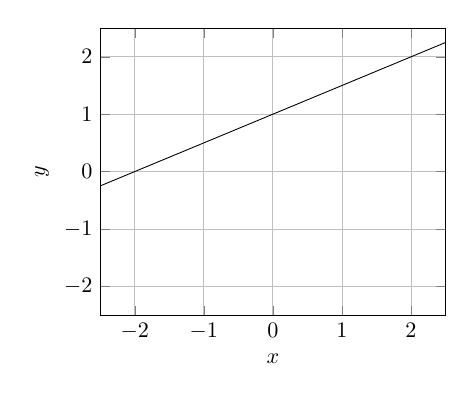
\begin{tikzpicture}[scale=0.8]
\begin{axis}[grid=both,
xmin=-2.5,xmax=2.5,
ymin=-2.5,ymax=2.5,
xtick={-2,...,2},
ytick={-2,...,2},
minor tick={},
xlabel=\(x\), ylabel=\(y\),
x post scale = 0.8,
y post scale = 0.8
]
\addplot[domain=-2.5:2.5] {1/2*x+1};

\end{axis}
\end{tikzpicture}
\end{center}

b)

\begin{center}
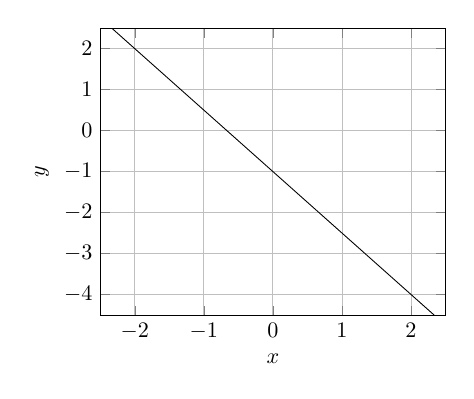
\begin{tikzpicture}[scale=0.8]
\begin{axis}[grid=both,
xmin=-2.5,xmax=2.5,
ymin=-4.5,ymax=2.5,
xtick={-2,...,2},
ytick={-4,...,2},
minor tick={},
xlabel=\(x\), ylabel=\(y\),
x post scale = 0.8,
y post scale = 0.8
]
\addplot[domain=-2.5:2.5] {-3/2*x-1};

\end{axis}
\end{tikzpicture}
\end{center}
 


\end{minipage}
\begin{minipage}[c]{0.5\textwidth}

c) 
\begin{center}
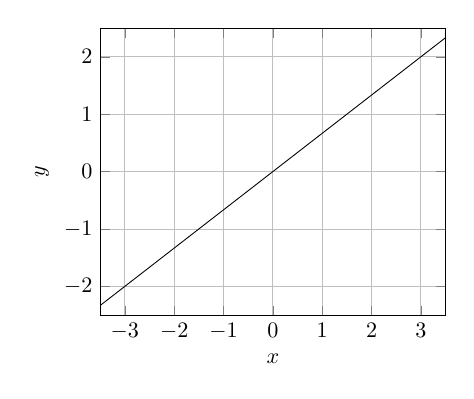
\begin{tikzpicture}[scale=0.8]
\begin{axis}[grid=both,
xmin=-3.5,xmax=3.5,
ymin=-2.5,ymax=2.5,
xtick={-3,...,3},
ytick={-2,...,2},
minor tick={},
xlabel=\(x\), ylabel=\(y\),
x post scale = 0.8,
y post scale = 0.8
]
\addplot[domain=-3.5:3.5] {2/3*x};

\end{axis}
\end{tikzpicture}
\end{center}


d)
\begin{center}
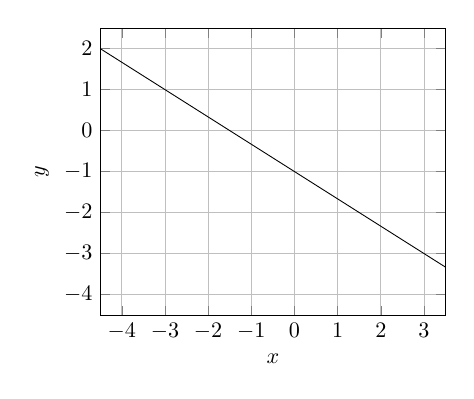
\begin{tikzpicture}[scale=0.8]
\begin{axis}[grid=both,
xmin=-4.5,xmax=3.5,
ymin=-4.5,ymax=2.5,
xtick={-4,...,3},
ytick={-4,...,2},
minor tick={},
xlabel=\(x\), ylabel=\(y\),
x post scale = 0.8,
y post scale = 0.8
]
\addplot[domain=-4.5:3.5] {-2/3*x-1};

\end{axis}
\end{tikzpicture}
\end{center}


\end{minipage}
\end{exercise}

\begin{solution}
    \begin{parts}
        \item slope: 0.5; vertical intercept: 1; equation: $y=0.5x+1$
        \item slope: $-\frac{3}{2}$; vertical intercept: $-1$; equation: $y=-\frac{3}{2}x-1$
        \item slope: $\frac{2}{3}$; vertical intercept: 0; equation: $y=\frac{2}{3}x$
        \item slope: $-\frac{2}{3}$; vertical intercept: $-1$; equation: $y=-\frac{2}{3}x-1$
    \end{parts}
\end{solution}






\newpage

\begin{exercise}
Five linear functions (a)-(e) are given below. Match each function with its graph from the figure to the right.
\\\begin{minipage}[c]{0.25\textwidth}
\begin{parts}
\item $y=-2x-3$
\item $y=3x-1$
\item $y=3x+2$
\item $y=x-1$
\item $y=2$
\end{parts}
\end{minipage}\begin{minipage}[c]{0.7\textwidth}


\begin{center}
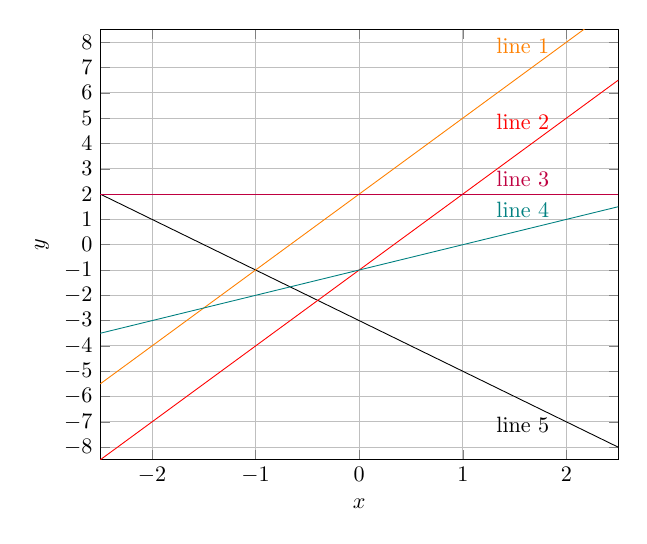
\begin{tikzpicture}[scale=0.8]
\begin{axis}[grid=both,
xmin=-2.5,xmax=2.5,
ymin=-8.5,ymax=8.5,
xtick={-2,...,2},
ytick={-8,...,8},
minor tick={},
xlabel=\(x\), ylabel=\(y\),
x post scale = 1.2,
y post scale = 1.2
]
\addplot[domain=-2.5:2.5] {-2*x-3} node[pos=0.85, below] {\hspace*{-16pt}line 5};
\addplot[domain=-2.5:2.5,red] {3*x-1} node[pos=0.85, above] {\hspace*{-16pt}line 2};
\addplot[domain=-2.5:2.5,orange] {3*x+2} node[pos=0.85, above] {\hspace*{-16pt}line 1};
\addplot[domain=-2.5:2.5,teal] {x-1} node[pos=0.85, above] {\hspace*{-16pt}line 4};
\addplot[domain=-2.5:2.5,purple] {2} node[pos=0.85, above] {\hspace*{-16pt}line 3};

\end{axis}
\end{tikzpicture}
\end{center}

\end{minipage}



\end{exercise}


\begin{solution}
    (a) is line 5; (b) is line 2; (c) is line 1; (d) is line 4; (e) is line 3
\end{solution}





\begin{exercise}
During the 2019-2020 academic year, a senior lecturer at URI earned a base salary of \$55,683 for a standard teaching load. For each credit taught in excess of the standard load, \$1,567 were added to his salary. Write a linear equation expressing the total amount $A$ that the senior lecturer earned for teaching $n$ credits in excess of the standard workload during the 2019-2020 academic year. 
\end{exercise}

\begin{solution}
$A=1567n+55683$
\end{solution}




\begin{exercise}
The elevation in feet, $E(t)$, of a hiker $t$ minutes after beginning her hike is given by $E(t)=35t+1350$.
\begin{parts}
\item Write a complete sentence explaining the practical meaning of the vertical intercept of this linear function. Include units in your answer.

\item Write a complete sentence explaining the practical meaning of the slope of this linear function. Include units in your answer.
\end{parts}
\end{exercise}


\begin{solution}
    \begin{parts}
        \item The initial elevation of the hiker is 1350 feet.
        \item The hiker's elevation is increasing at a rate of 35 feet per minute.
    \end{parts}
\end{solution}






\begin{exercise}
The distance in miles from the finish line, $D(t)$, of a bicyclist $t$ hours after beginning a race is given by $D(t)=50-25t$.
\begin{parts}
\item Write a complete sentence explaining the practical meaning of the vertical intercept of this linear function. Include units in your answer.
\item Write a complete sentence explaining the practical meaning of the slope of this linear function. Include units in your answer.
\end{parts}
\end{exercise}

\begin{solution}
    \begin{parts}
        \item The bicyclist's initial distance from the finish line is 50 miles.
        \item The bicyclist's distance from the finish line is decreasing at a rate of 25 miles per hour.
    \end{parts}
\end{solution}






